\chapter{系統概述} % Main chapter title
\label{chapter1} % For referencing the chapter elsewhere, use \ref{1_Chapter1}
\ifpdf
    \graphicspath{{Figures/chapter1/PNG/}{Figures/chapter1/PDF/}{Figures/chapter1/}}
\else
    \graphicspath{{Figures/chapter1/EPS/}{Figures/chapter1/}}
\fi


\section{主機狀況}\label{1_sec:define}
本機一切正常,並無出現特殊硬體錯誤與問題。

\subsection{硬體配備}\label{1_subsec:WCSGC}

\begin{itemize}
    \item CPU
    \item Memoy
    \item Graphic
    \item Hard Disk
    \item SSD
\end{itemize}

\begin{figure*}
    \centering
    \subfigure[]{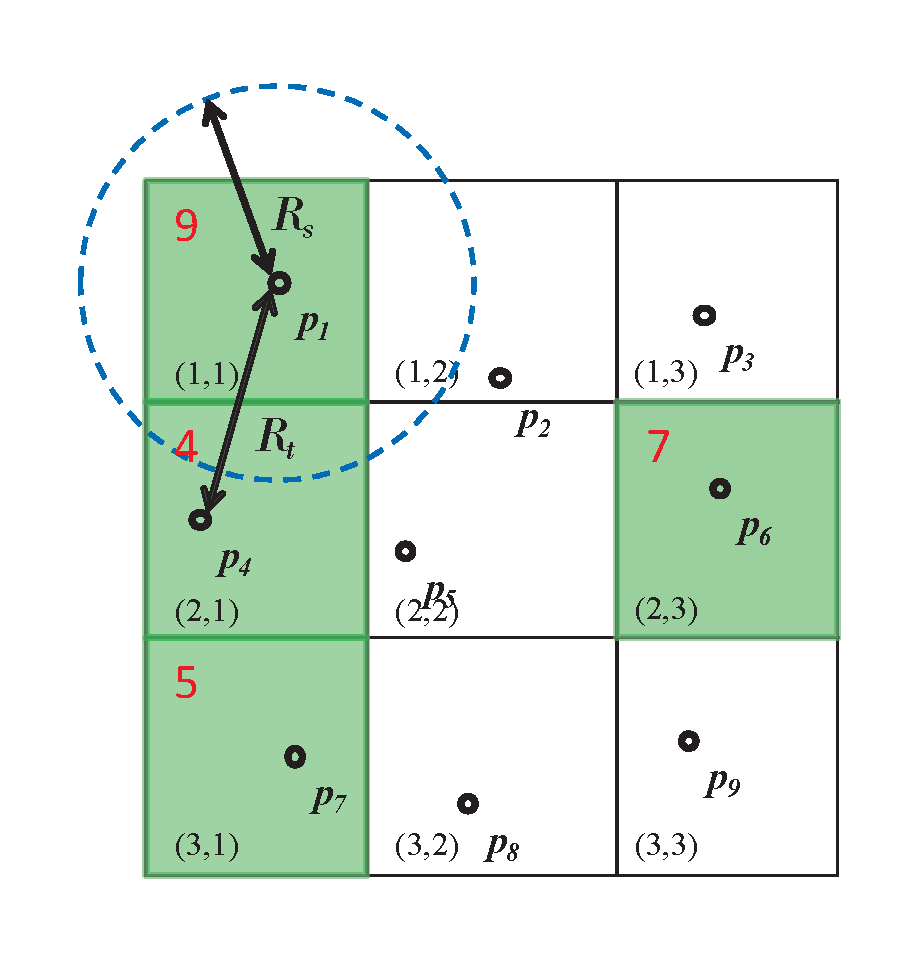
\includegraphics[width=6.5cm]{2a.eps}\label{1_fig_network_model:a}}
    \subfigure[]{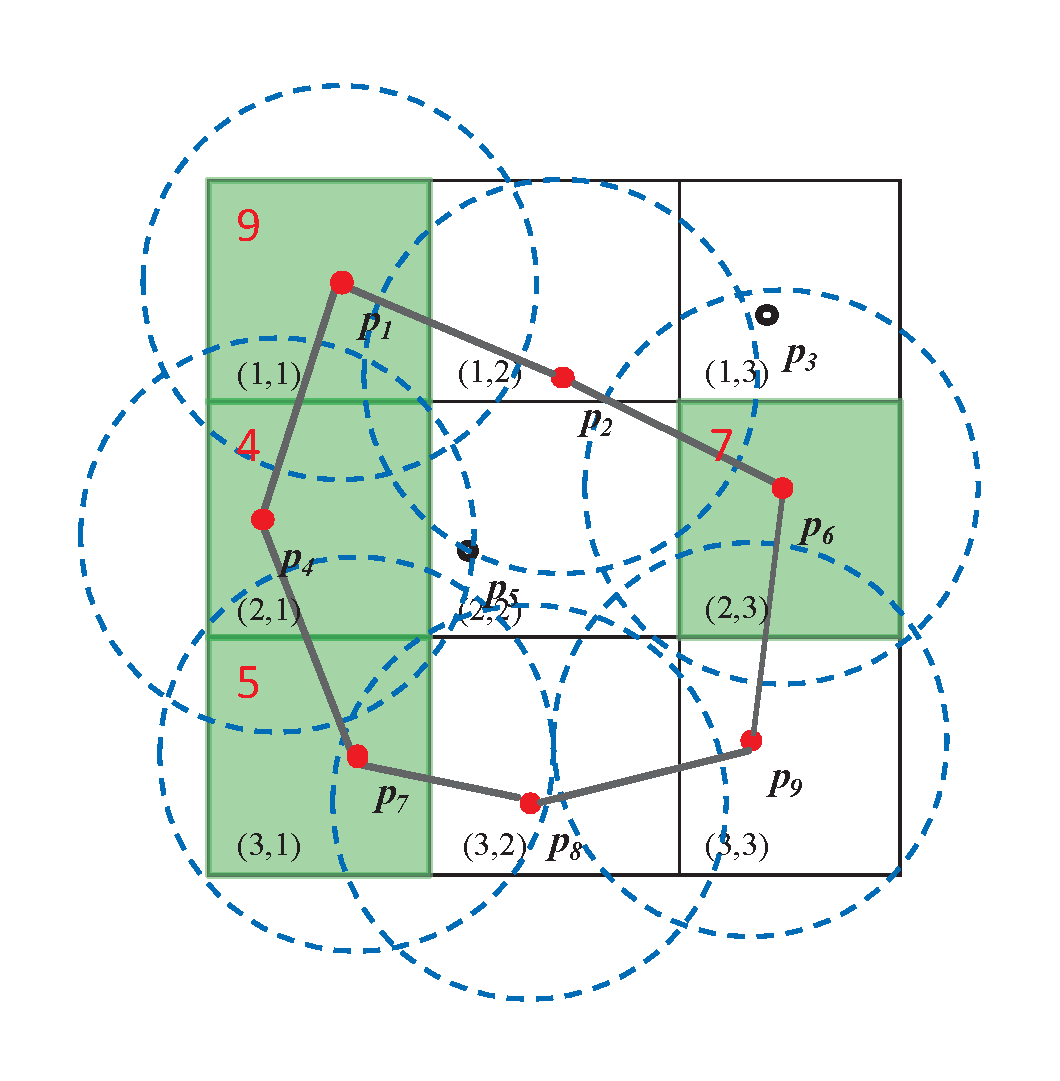
\includegraphics[width=7cm,height=7cm]{2b.eps}\label{1_fig_network_model:b}}
    \caption{Example of the
    weighted-critical-square-grid coverage problem. (a) A sensor field
    divided into $9$ grids of squares with length $\ell$, where
    $R_s=\frac{\sqrt{3}}{2}\ell$, $R_t=\ell$, every grid is labeled with
    a pair of numbers, four critical grids are labeled with $(1,1)$,
    $(2,1)$, $(2,3)$, and $(3,1)$ are shown in green, the weight of each
    critical grid is shown in red, and hollow circles are the points
    that are allowed to deploy sensors. (b) A wireless sensor network
    constructed by $7$ sensors denoted by solid circles, where an edge
    between two sensors represents that the two sensors can communicate
    with each other.} \label{1_fig_network_model}
\end{figure*}
